% Options for packages loaded elsewhere
\PassOptionsToPackage{unicode}{hyperref}
\PassOptionsToPackage{hyphens}{url}
\PassOptionsToPackage{dvipsnames,svgnames,x11names}{xcolor}
%
\documentclass[
  ignorenonframetext,
]{beamer}
\usepackage{pgfpages}
\setbeamertemplate{caption}[numbered]
\setbeamertemplate{caption label separator}{: }
\setbeamercolor{caption name}{fg=normal text.fg}
\beamertemplatenavigationsymbolsempty
% Prevent slide breaks in the middle of a paragraph
\widowpenalties 1 10000
\raggedbottom
\setbeamertemplate{part page}{
  \centering
  \begin{beamercolorbox}[sep=16pt,center]{part title}
    \usebeamerfont{part title}\insertpart\par
  \end{beamercolorbox}
}
\setbeamertemplate{section page}{
  \centering
  \begin{beamercolorbox}[sep=12pt,center]{part title}
    \usebeamerfont{section title}\insertsection\par
  \end{beamercolorbox}
}
\setbeamertemplate{subsection page}{
  \centering
  \begin{beamercolorbox}[sep=8pt,center]{part title}
    \usebeamerfont{subsection title}\insertsubsection\par
  \end{beamercolorbox}
}
\AtBeginPart{
  \frame{\partpage}
}
\AtBeginSection{
  \ifbibliography
  \else
    \frame{\sectionpage}
  \fi
}
\AtBeginSubsection{
  \frame{\subsectionpage}
}
\usepackage{amsmath,amssymb}
\usepackage{lmodern}
\usepackage{iftex}
\ifPDFTeX
  \usepackage[T1]{fontenc}
  \usepackage[utf8]{inputenc}
  \usepackage{textcomp} % provide euro and other symbols
\else % if luatex or xetex
  \usepackage{unicode-math}
  \defaultfontfeatures{Scale=MatchLowercase}
  \defaultfontfeatures[\rmfamily]{Ligatures=TeX,Scale=1}
\fi
% Use upquote if available, for straight quotes in verbatim environments
\IfFileExists{upquote.sty}{\usepackage{upquote}}{}
\IfFileExists{microtype.sty}{% use microtype if available
  \usepackage[]{microtype}
  \UseMicrotypeSet[protrusion]{basicmath} % disable protrusion for tt fonts
}{}
\makeatletter
\@ifundefined{KOMAClassName}{% if non-KOMA class
  \IfFileExists{parskip.sty}{%
    \usepackage{parskip}
  }{% else
    \setlength{\parindent}{0pt}
    \setlength{\parskip}{6pt plus 2pt minus 1pt}}
}{% if KOMA class
  \KOMAoptions{parskip=half}}
\makeatother
\usepackage{xcolor}
\newif\ifbibliography
\usepackage{graphicx}
\makeatletter
\def\maxwidth{\ifdim\Gin@nat@width>\linewidth\linewidth\else\Gin@nat@width\fi}
\def\maxheight{\ifdim\Gin@nat@height>\textheight\textheight\else\Gin@nat@height\fi}
\makeatother
% Scale images if necessary, so that they will not overflow the page
% margins by default, and it is still possible to overwrite the defaults
% using explicit options in \includegraphics[width, height, ...]{}
\setkeys{Gin}{width=\maxwidth,height=\maxheight,keepaspectratio}
% Set default figure placement to htbp
\makeatletter
\def\fps@figure{htbp}
\makeatother
\setlength{\emergencystretch}{3em} % prevent overfull lines
\providecommand{\tightlist}{%
  \setlength{\itemsep}{0pt}\setlength{\parskip}{0pt}}
\setcounter{secnumdepth}{-\maxdimen} % remove section numbering

\usepackage{textpos}
\setbeamertemplate{headline}{
  \begin{textblock*}{5cm}(10.2cm,0.2cm)
  
\includegraphics[width=2.2cm]{UniUrb-logo.png}
  \end{textblock*}}
  
  
  \definecolor{myblue}{HTML}{005997}
  \setbeamercolor{frametitle}{fg=myblue}
    \setbeamercolor{framesubtitle}{fg=myblue}
    \setbeamercolor{frametitle right}{fg=myblue}
  \setbeamercolor{titlelike}{fg=myblue}
    \setbeamercolor{title}{fg=myblue}
      \setbeamercolor{subtitle}{fg=myblue}
    \setbeamercolor{part title}{fg=myblue}
    \setbeamercolor{section title}{fg=myblue}
    \setbeamercolor{subsection title}{fg=myblue}
  \setbeamercolor{section name}{fg=myblue}
  \setbeamercolor{subsection name}{fg=myblue}
  \setbeamercolor{part name}{fg=myblue}
  \setbeamercolor{title in head/foot}{fg=myblue}
  \setbeamercolor{subtitle in head/foot}{fg=myblue}
  \setbeamercolor{block title}{fg=myblue}
  
  \setbeamercolor{bullet}{fg=myblue}
  \setbeamercolor{section in toc}{fg=myblue}
  \setbeamercolor{subsection in toc}{fg=myblue}
  \setbeamercolor{section in head/foot}{fg=myblue}
  \setbeamercolor{subsection in head/foot}{fg=myblue}
  
  
  \setbeamercolor{itemize item}{fg = myblue}
  \setbeamercolor{itemize subitem}{fg = myblue}
  \setbeamercolor{itemize subsubitem}{fg = myblue}
  \setbeamercolor{enumerate item}{fg = myblue}
  \setbeamercolor{enumerate subitem}{fg = myblue}
  \setbeamercolor{enumerate subsubitem}{fg = myblue}
  
 
  
\usepackage{etoolbox}
\AtBeginEnvironment{thebibliography}{\scriptsize}
\ifLuaTeX
  \usepackage{selnolig}  % disable illegal ligatures
\fi
\usepackage[round]{natbib}
\bibliographystyle{apalike}
\IfFileExists{bookmark.sty}{\usepackage{bookmark}}{\usepackage{hyperref}}
\IfFileExists{xurl.sty}{\usepackage{xurl}}{} % add URL line breaks if available
\urlstyle{same} % disable monospaced font for URLs
\hypersetup{
  pdftitle={Bibliometric Analysis of European Research on Digital Divide: An Exploration of the Corporate Landscape},
  pdfauthor={Luis Carlos Castillo},
  colorlinks=true,
  linkcolor={myblue},
  filecolor={Maroon},
  citecolor={Blue},
  urlcolor={Blue},
  pdfcreator={LaTeX via pandoc}}

\title{Bibliometric Analysis of European Research on Digital Divide: An
Exploration of the Corporate Landscape}
\author{Luis Carlos Castillo}
\date{20 June 2023}
\institute{Supervisor: Prof.~Francesco Vidoli\\
University of Urbino\\
Ph.D.~Program in Global Studies}

\begin{document}
\frame{\titlepage}

\begin{frame}{Content I}
\protect\hypertarget{content-i}{}
\begin{enumerate}
\item
  Digital Divide Overview
\item
  Motivation
\item
  Research Questions
\item
  Data
\item
  Bibliometric Analysis
\end{enumerate}
\end{frame}

\begin{frame}{Content II}
\protect\hypertarget{content-ii}{}
\begin{enumerate}
\setcounter{enumi}{5}
\item
  Performance Analysis

  \begin{enumerate}
  \tightlist
  \item
    Publications Vs Citations
  \item
    Authors
  \item
    Articles
  \item
    Journals
  \item
    Affiliations/ Universities
  \item
    Countries
  \end{enumerate}
\item
  Science Mapping

  \begin{enumerate}
  \tightlist
  \item
    Citations Analysis
  \item
    Similarity Measures

    \begin{enumerate}
    \tightlist
    \item
      Co-citations Analysis
    \item
      Bibliographic Coupling
    \end{enumerate}
  \end{enumerate}
\item
  Conclusions
\end{enumerate}
\end{frame}

\begin{frame}{1. The Digital Divide Overview I}
\protect\hypertarget{the-digital-divide-overview-i}{}
\begin{itemize}
\tightlist
\item
  The digital divide is also known as the digital gap, inequalities, or
  disparities.
\item
  The interaction with other existing gaps such as income, education,
  gender, age, and regional, among others \citep{ragnedda2017}.
\item
  The evolution of the concept has pointed out the phenomenon's
  complexity and the effects on the different layers of society and the
  economy \citep{vandijk2003, ragnedda2017, shakina2021}.
\end{itemize}
\end{frame}

\begin{frame}{1. The Digital Divide Overview II}
\protect\hypertarget{the-digital-divide-overview-ii}{}
\begin{itemize}
\tightlist
\item
  Waves of Research

  \begin{itemize}
  \item
    \textbf{The first wave:} Physical access to technology
    -\textgreater{} possession of computers and access to the internet
    \citep{norris2001, james2002, castells2003}.
  \item
    \textbf{The second wave:} Usage of digital technologies and skills
    \citep{hargittai2002b, vandijk2005b, vandijk2006c, vandeursen2011c}.
  \item
    \textbf{The third wave:} The disparities in tangible outcomes arise
    from different forms of access to and usage of digital technologies,
    emphasizing the ability to benefit from these technologies in a
    data-driven market to enhance personal and professional aspects
    \citep{ragnedda2017, vandeursen2015a}.
  \end{itemize}
\end{itemize}
\end{frame}

\begin{frame}{1. The digital divide overview III}
\protect\hypertarget{the-digital-divide-overview-iii}{}
\begin{block}{The corporate landscape}
\protect\hypertarget{the-corporate-landscape}{}
\begin{itemize}
\tightlist
\item
  Digital revolution -\textgreater{} different aspects of daily
  activities -\textgreater{} how we conduct business.
\item
  Disparity in digital capabilities and resources among businesses
  \citep{shakina2021}.
\item
  The corporate digital divide is a topic that remains under-explored
  \citep{pejicbach2013, shakina2021}.
\item
  Understanding and addressing the divide, policymakers, and businesses
  owners can target their efforts to ensure inclusive digital
  transformation.
\end{itemize}
\end{block}
\end{frame}

\begin{frame}{2. Motivation}
\protect\hypertarget{motivation}{}
\begin{itemize}
\item
  Investigating the transformative effects of digital technologies on
  society and economy, while highlighting both opportunities and
  challenges.
\item
  Aligning with the Digital Europe program's vision by devising
  strategies to bridge the digital divide effectively.
\item
  Diversifying bibliometric research by extending its application beyond
  health sciences, computer science, and technology to understand the
  digital divide.
\item
  Harnessing the power of comprehensive data from three leading academic
  platforms to generate insightful and actionable findings on the
  digital divide.
\end{itemize}
\end{frame}

\begin{frame}{3. Research Questions}
\protect\hypertarget{research-questions}{}
\begin{block}{Research Questions}
\protect\hypertarget{research-questions-1}{}
\begin{itemize}
\item
  Q1: How have the main trends, focus shifts, and key themes in European
  research on the digital divide evolved over time, and how do they
  reflect the current state of knowledge in this field?
\item
  Q2: What are the intellectual interactions and thematic relationships
  among European research components on the digital divide, and how do
  they contribute to the identification of core subtopics and literature
  clusters?
\item
  Q3: How are European studies addressing the corporate digital divide,
  and which unexplored topics within this domain warrant further
  examination?
\end{itemize}
\end{block}
\end{frame}

\begin{frame}{4. Data I}
\protect\hypertarget{data-i}{}
\begin{itemize}
\tightlist
\item
  Specific search within titles and author keywords on the
  ``\emph{digital divide}'' merging data from the Web of Science,
  Scopus, and Dimensions platforms.
\item
  Search criteria: ``digital divide*'' OR ``digital inequalit*'' OR
  ``digital gap*''
\item
  The sample includes articles, book chapters, conferences, and
  proceeding papers.
\item
  Authors with European affiliations within the \textbf{business,
  management, economics, technology, and computer science} disciplines
  were included
\end{itemize}
\end{frame}

\begin{frame}{4. Data II}
\protect\hypertarget{data-ii}{}
\begin{itemize}
\item
  After conducting a thorough data cleaning, a total of 1609 unique
  documents from 2000 to 2022 were incorporated.
\item
  Number of Documents by Database

  \begin{itemize}
  \tightlist
  \item
    WoS:946
  \item
    Scopus: 254
  \item
    Dimensions: 409
  \end{itemize}
\item
  To track the evolution of the digital divide literature, the data was
  divided into three periods: 2000-2007, 2008-2015, and 2016-2022.
\item
  The R programming language environment.
\item
  To ensure both replicability and reproducibility, a public repository
  named ``dd\_bibliometric\_europe'' has been established on GitHub.
\end{itemize}
\end{frame}

\begin{frame}{5. Methodology I}
\protect\hypertarget{methodology-i}{}
\begin{block}{Bibliometric Analysis}
\protect\hypertarget{bibliometric-analysis}{}
Following \citet{donthu2021}, \citet{Aria2017}, \citet{ellegaard2015}
and \citet{Bornmann2015} bibliometric analysis:

\begin{itemize}
\tightlist
\item
  Is a methodology that applies quantitative techniques to bibliographic
  data and plays a vital role in evaluating research output.
\item
  This technique allows researchers to uncover emerging trends
  identifying knowledge gaps in specific domains and analyze a
  significant quantity of documents .
\item
  It offers three types of analysis: performance analysis, science
  mapping, and network analysis.
\end{itemize}
\end{block}
\end{frame}

\begin{frame}{6. Performance Analysis I}
\protect\hypertarget{performance-analysis-i}{}
Is a descriptive interpretation of research constituents.

\begin{block}{6.1. Publications vs Citations}
\protect\hypertarget{publications-vs-citations}{}
\vspace{0.5cm}

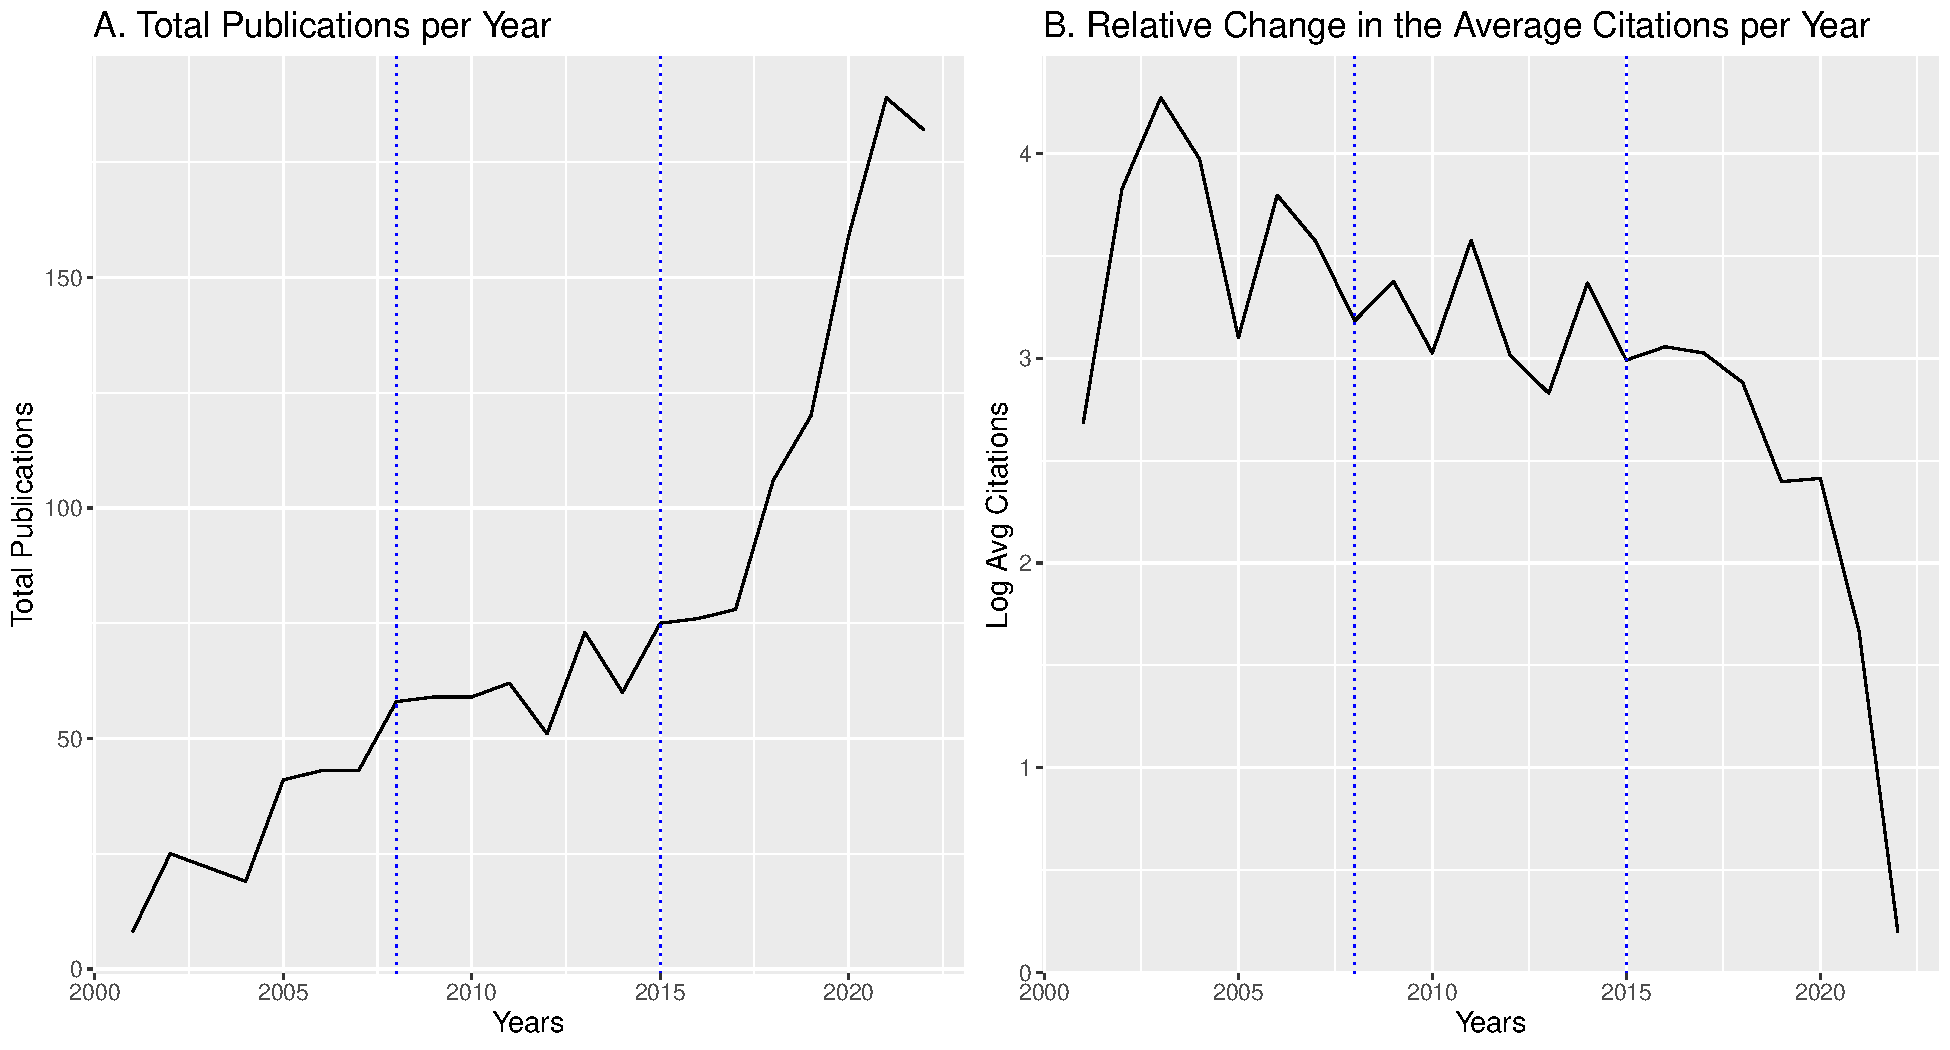
\includegraphics{Presentation_bibliometric_Madrid_june_20_files/figure-beamer/Panel cite vs prod-1.pdf}
\end{block}
\end{frame}

\begin{frame}{6. Performance Analysis II}
\protect\hypertarget{performance-analysis-ii}{}
\vspace{0.5cm}

\begin{center}
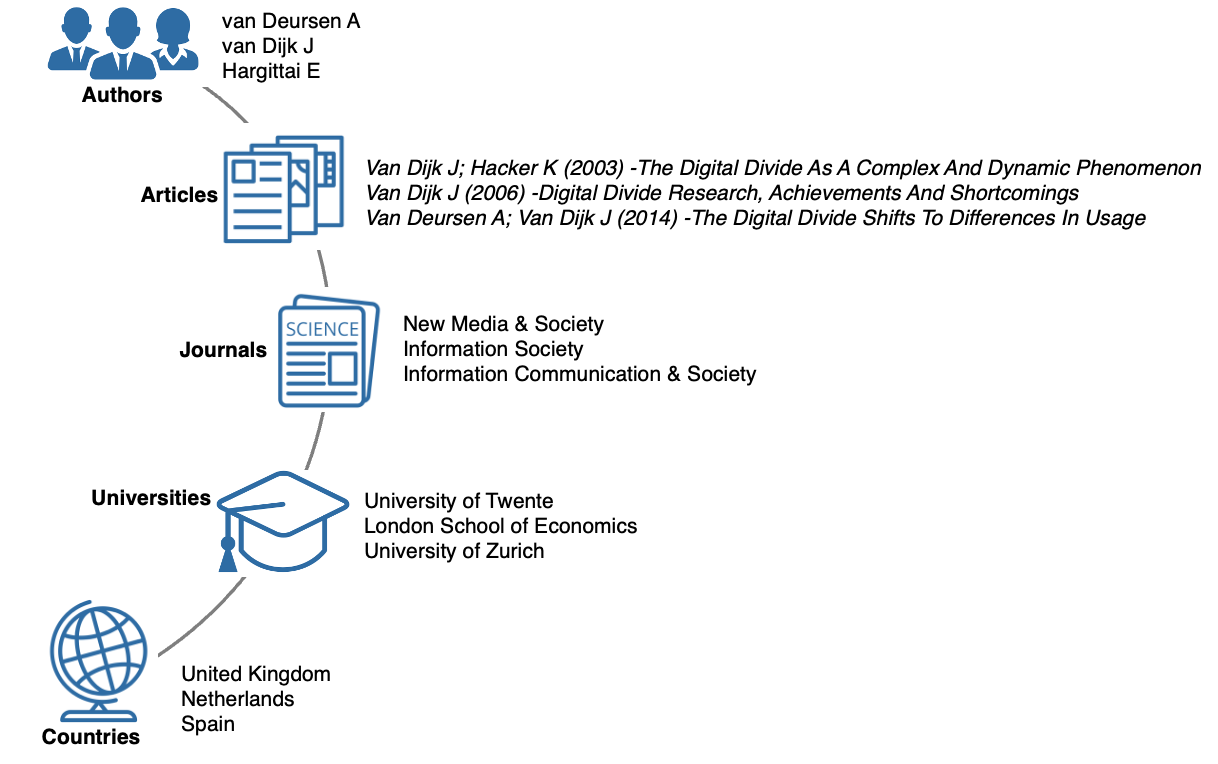
\includegraphics[width=1\textwidth]{pic_2.png}
\end{center}
\end{frame}

\begin{frame}{7. Science Mapping I}
\protect\hypertarget{science-mapping-i}{}
\begin{block}{7.2. Similarity measures}
\protect\hypertarget{similarity-measures}{}
Quantify similarity, connections and relationships among academic
entities.

Following \citet{kammerer2021}

\begin{itemize}
\item
  \textbf{Knowledge base:} cluster of academic publications in a
  research field that are considered fundamental to the development and
  understanding of the field.
\item
  \textbf{Research front:} cluster of academic publications that refers
  to emerging active areas of research considering themselves with a
  similar unsolved research problem.
\end{itemize}

\begin{center}
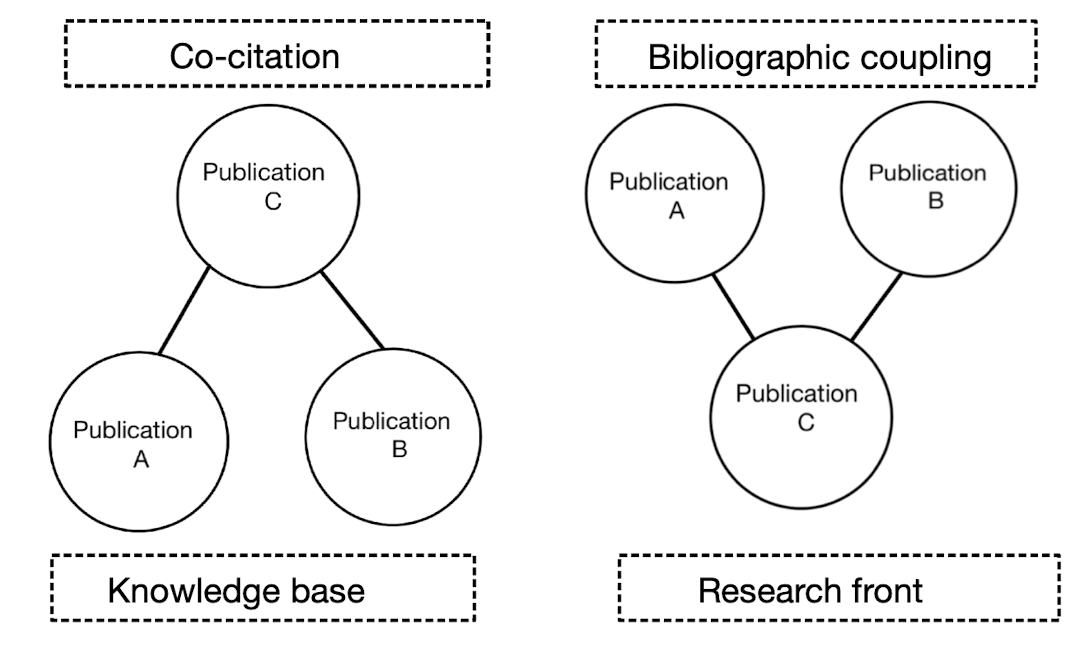
\includegraphics[width=0.6\textwidth]{pic_1.png}
\end{center}
\end{block}
\end{frame}

\begin{frame}{7. Science Mapping II}
\protect\hypertarget{science-mapping-ii}{}
\vspace{0.5cm}

\begin{block}{7.2.1. Co-citations Analyisis}
\protect\hypertarget{co-citations-analyisis}{}
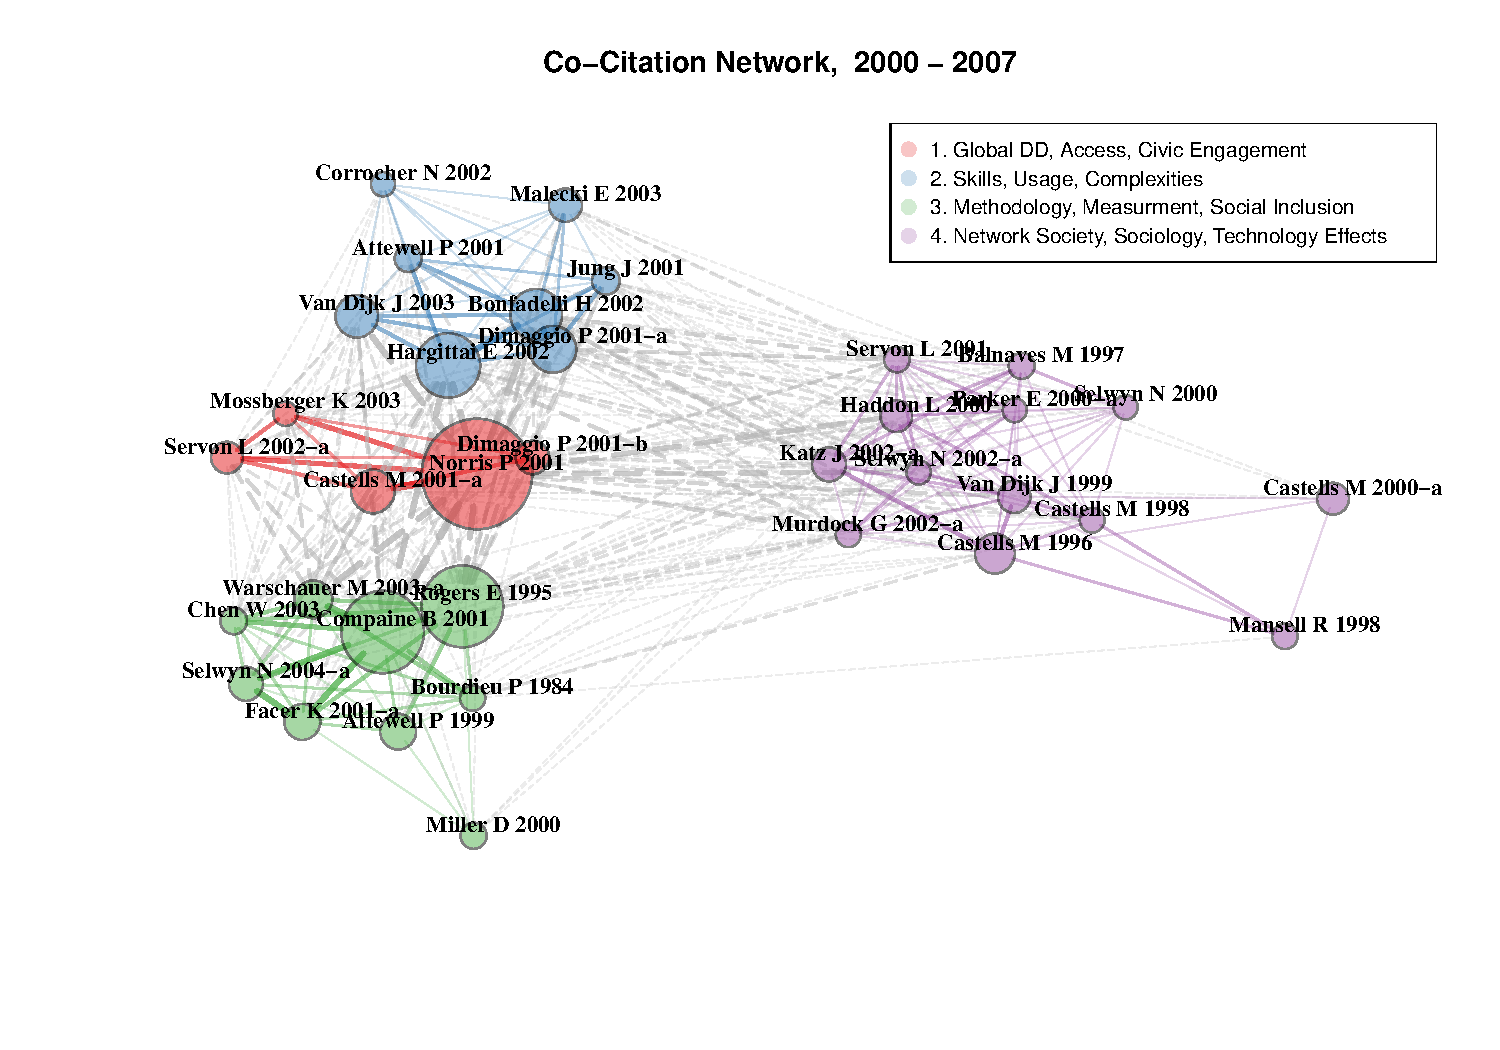
\includegraphics{Presentation_bibliometric_Madrid_june_20_files/figure-beamer/Co_cite_P1-1.pdf}
\end{block}
\end{frame}

\begin{frame}{7. Science Mapping III}
\protect\hypertarget{science-mapping-iii}{}
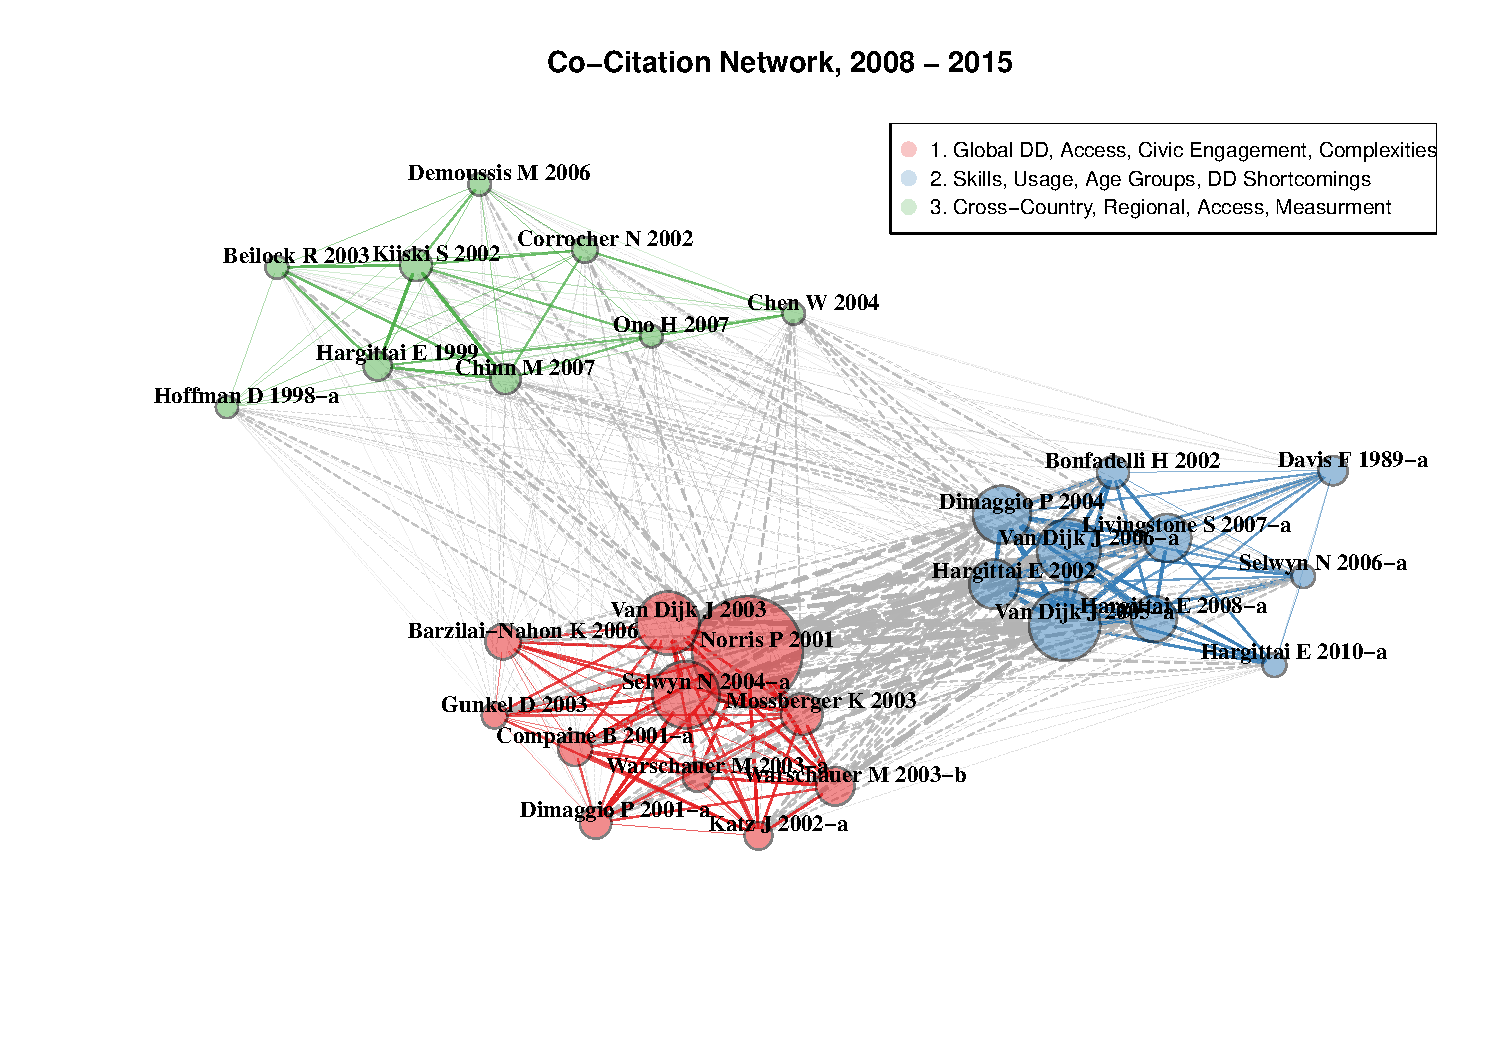
\includegraphics{Presentation_bibliometric_Madrid_june_20_files/figure-beamer/Co_cite_P2-1.pdf}
\end{frame}

\begin{frame}{7. Science Mapping IV}
\protect\hypertarget{science-mapping-iv}{}
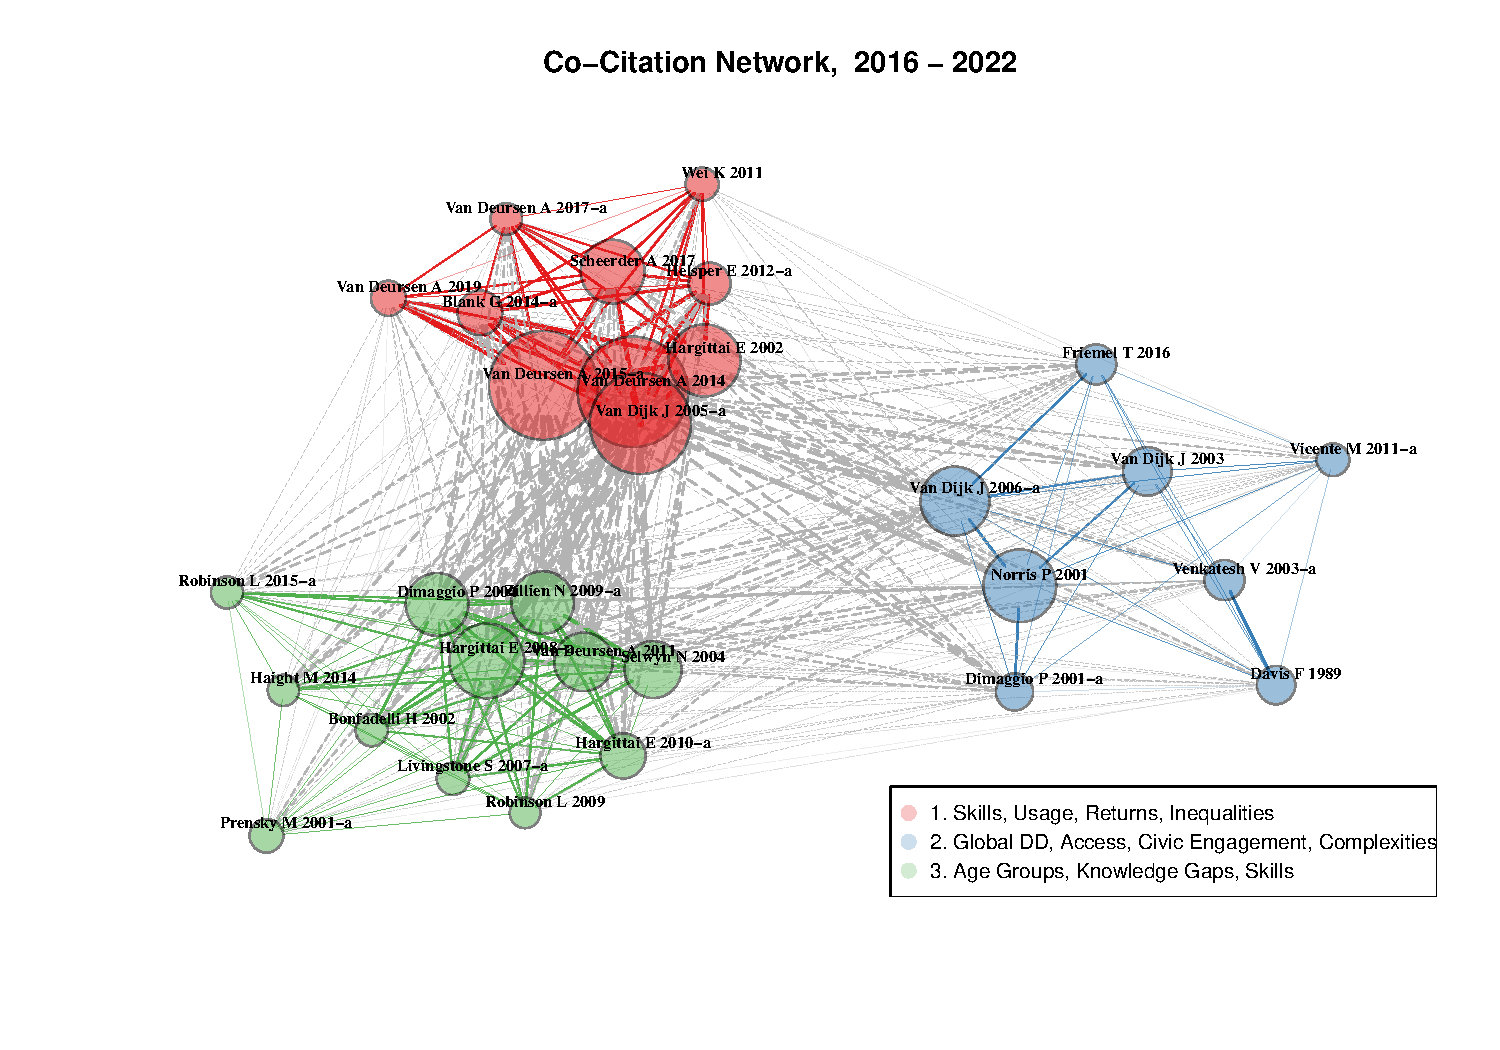
\includegraphics{Presentation_bibliometric_Madrid_june_20_files/figure-beamer/Co_cite_P3-1.pdf}
\end{frame}

\begin{frame}{7. Science Mapping V}
\protect\hypertarget{science-mapping-v}{}
\begin{block}{Co-citation Networks Summary}
\protect\hypertarget{co-citation-networks-summary}{}
This three networks highlighted:

\begin{itemize}
\item
  \textbf{Evolution of research focus:} From internet access and
  methodological focus to the various facets of the digital divide.
\item
  \textbf{Key publications and intellectual interactions:} Norris
  (2001), van Dijk (2005) Hargittai (2002) and van Deursen and van Dijk
  (2014) shape the discourse and the intellectual interactions.
\item
  \textbf{Emerging trends and themes:} The third-level digital divide
  and its broader socio-economic ramifications. Uncovering a research
  gap remains unexplored concerning the corporate digital divide.
\end{itemize}
\end{block}
\end{frame}

\begin{frame}{7. Science Mapping VI}
\protect\hypertarget{science-mapping-vi}{}
\begin{block}{7.2.2. Bibliographic Coupling Analysis}
\protect\hypertarget{bibliographic-coupling-analysis}{}
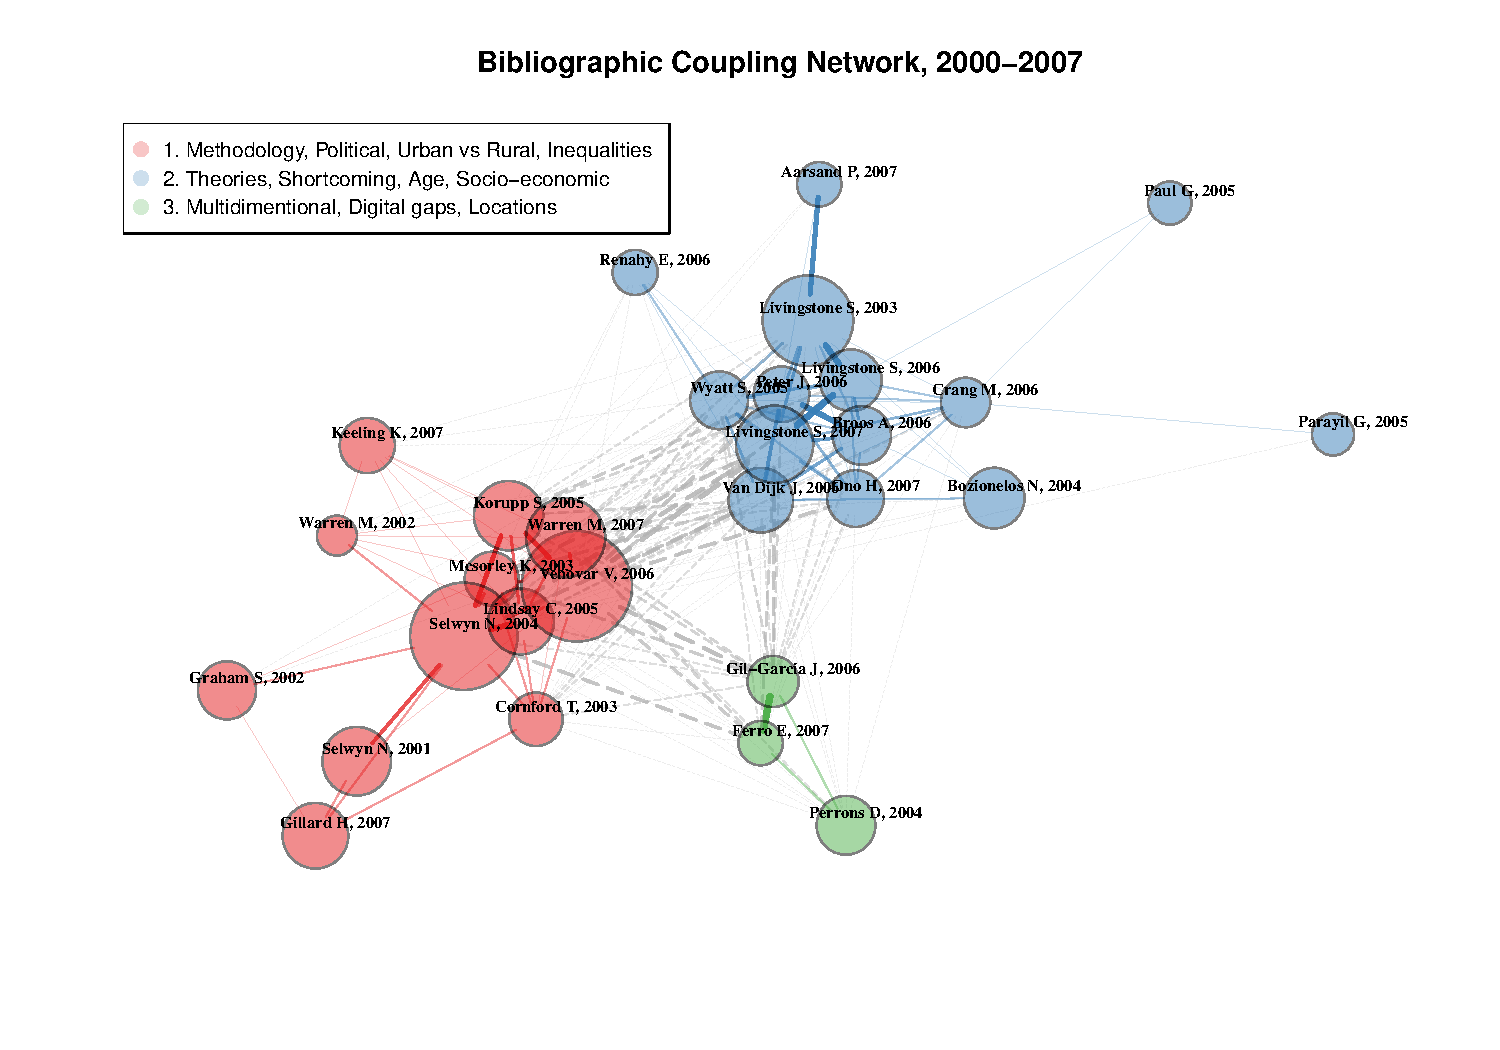
\includegraphics{Presentation_bibliometric_Madrid_june_20_files/figure-beamer/Bib_coup_P1-1.pdf}
\end{block}
\end{frame}

\begin{frame}{7. Science Mapping VII}
\protect\hypertarget{science-mapping-vii}{}
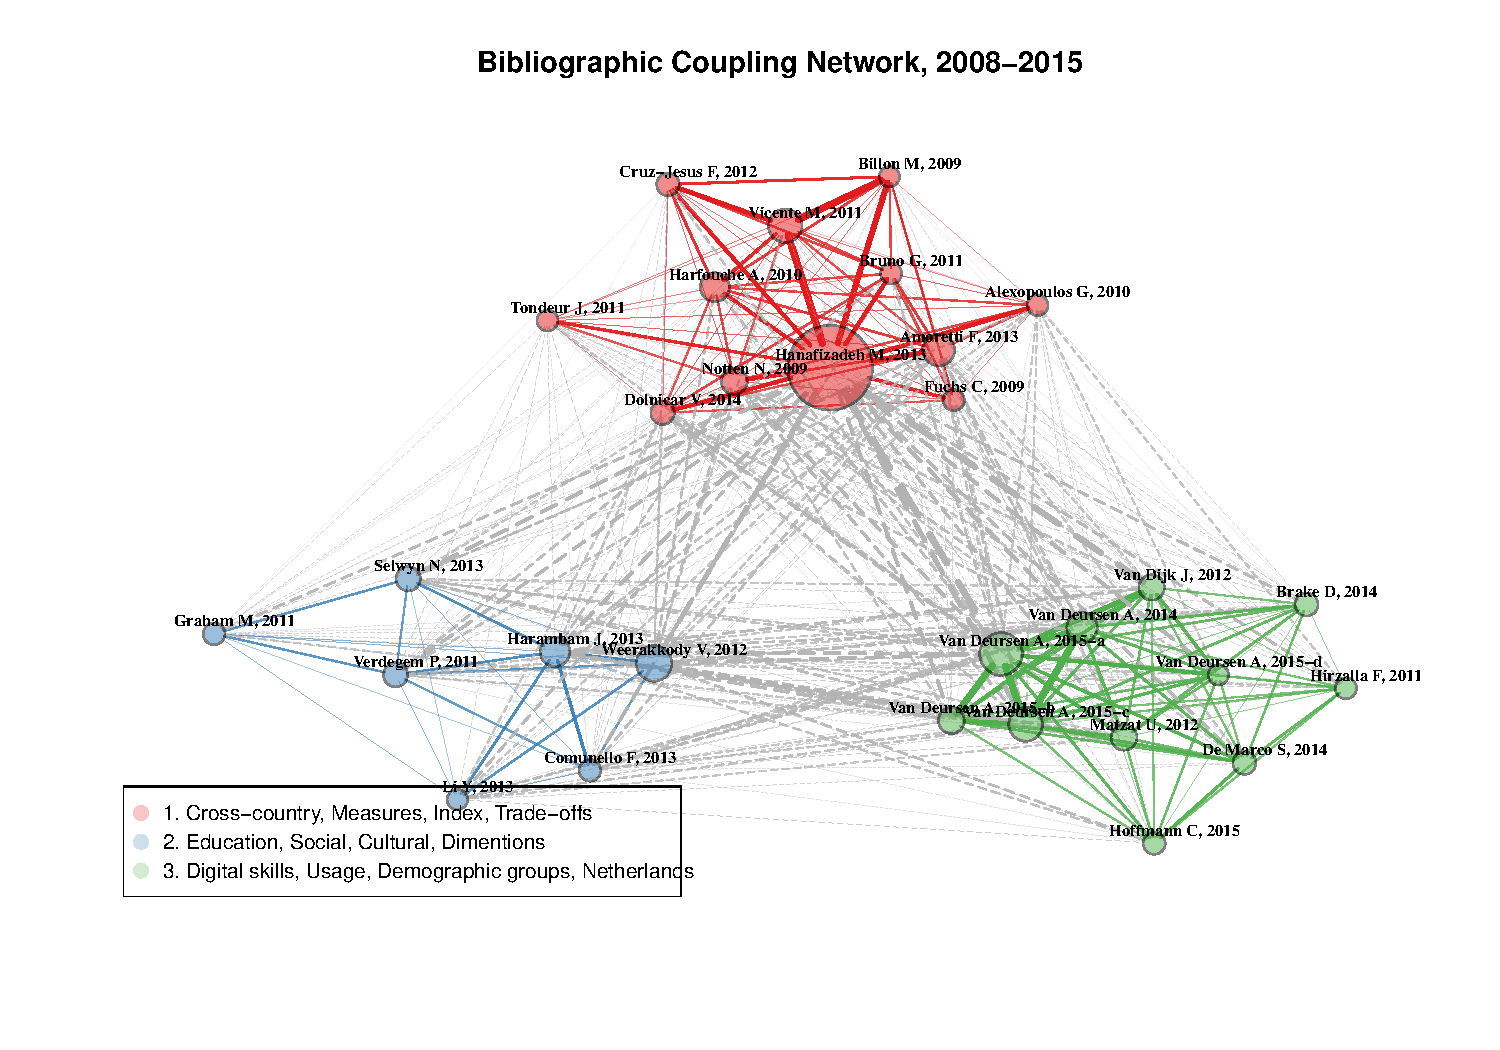
\includegraphics{Presentation_bibliometric_Madrid_june_20_files/figure-beamer/Bib_coup_P2-1.pdf}
\end{frame}

\begin{frame}{7. Science Mapping VIII}
\protect\hypertarget{science-mapping-viii}{}
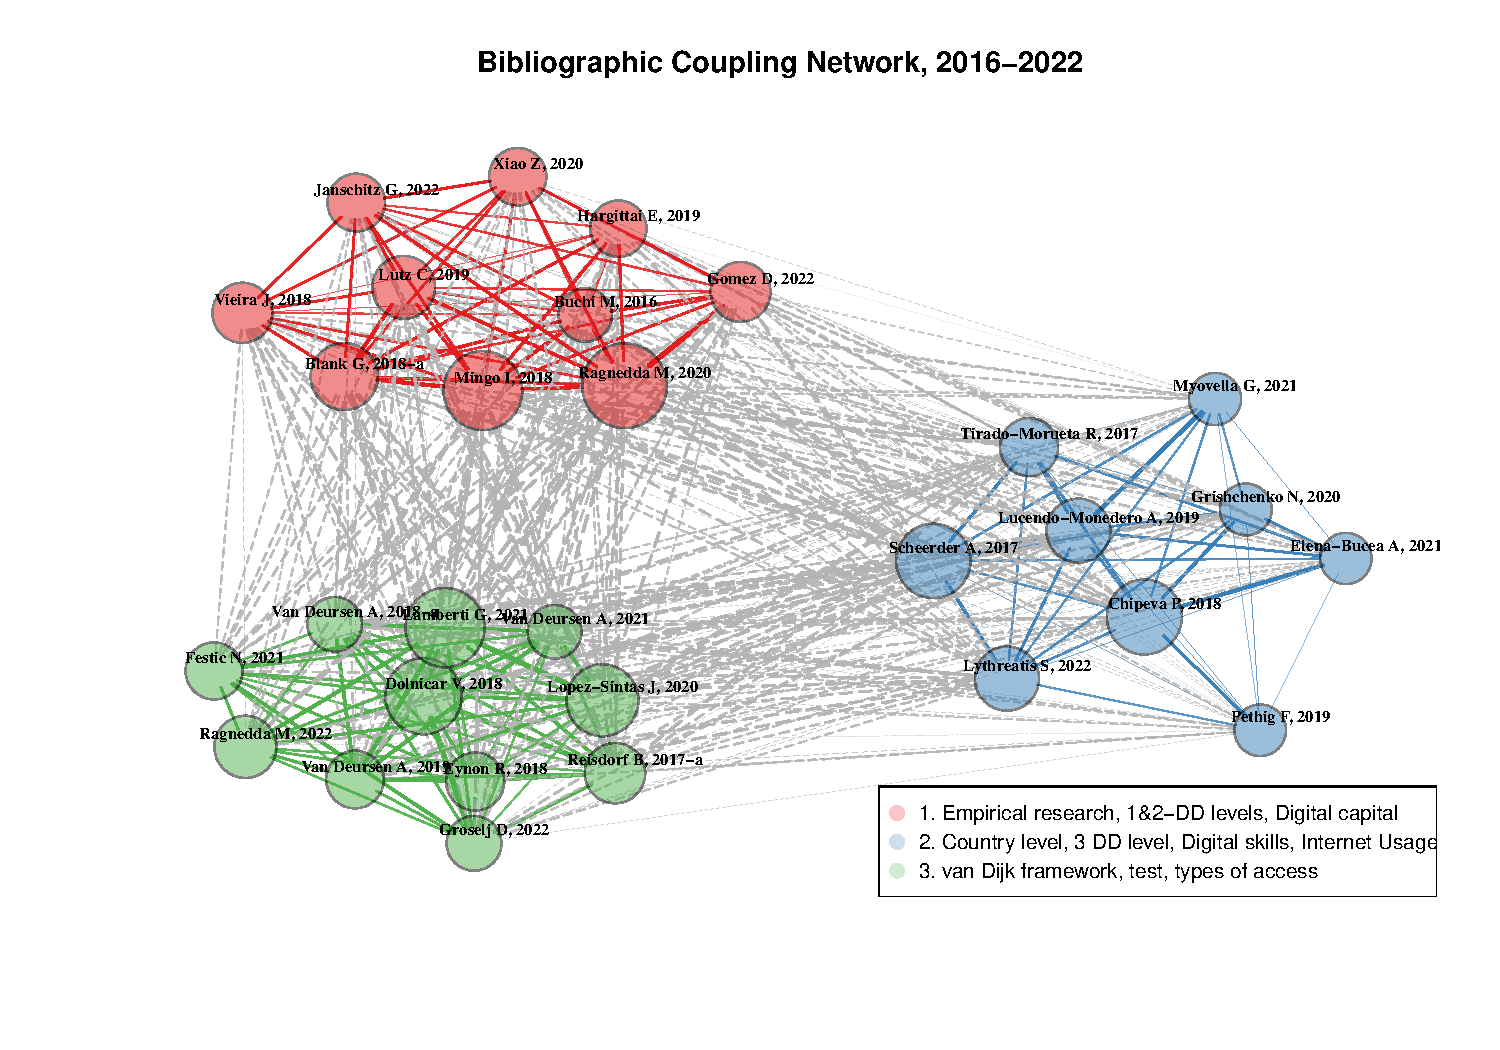
\includegraphics{Presentation_bibliometric_Madrid_june_20_files/figure-beamer/Bib_coup_P3-1.pdf}
\end{frame}

\begin{frame}{7. Science Mapping IX}
\protect\hypertarget{science-mapping-ix}{}
\begin{block}{Bibliographic coupling Networks Summary}
\protect\hypertarget{bibliographic-coupling-networks-summary}{}
This three networks highlighted:

\begin{itemize}
\item
  \textbf{Evolution of unsolved research problems:} From political,
  methodological challenges, regional analysis to cross-country
  analysis, measurements shortcomings and testing the theory.
\item
  \textbf{Emergence of key authors and publications:} Prominent
  publications by authors such as Van Dijk, van Deursen, and
  Livingstone, featured prominently across clusters, represent the
  intellectual interactions of the research front.
\item
  \textbf{Growing complexities and specialization:} The diverse research
  themes in the networks reflect the expanding scope and depth of
  digital divide research. The last BC network illustrates the current
  state of research.
\end{itemize}
\end{block}
\end{frame}

\begin{frame}{Conclusions}
\protect\hypertarget{conclusions}{}
\begin{itemize}
\item
  The intellectual structure of the knowledge base and research front in
  the digital divide is evolving but it need further development
  regarding the use of latest technologies.
\item
  The networks showcase intellectual interactions among prominent
  authors and publications that consistently contribute in the field.
  The thematic relationships lead to the current state of research.
\item
  European studies have not extensively addressed the corporate digital
  divide, leaving room for further examination. The corporate digital
  divide might be incorporated into other literature streams, such as
  digital transformation, technology adoption, and knowledge management.
\end{itemize}
\end{frame}

\begin{frame}{Contact information}
\protect\hypertarget{contact-information}{}
\vspace{2cm}

Luis Carlos Castillo-Tellez

\vspace{0.1cm}

PhD candidate in Global Studies

University of Urbino - Italy

email:
\href{mailto:l.castillotellez@campus.uniurb.it}{\nolinkurl{l.castillotellez@campus.uniurb.it}}
\end{frame}

\renewcommand\refname{References}
\begin{frame}[allowframebreaks]{References}
  \bibliographytrue
  \bibliography{references.bib}
\end{frame}

\end{document}
